\documentclass[11pt]{article}

%defines page size and margins
\usepackage{geometry}
\geometry{
    letterpaper,
    left=1in,
    right=1in,
    top=1in,
    bottom=1in,
}

%Sets spacing for entire document
\usepackage{setspace}
\singlespacing

%Package for reducing space in between list items
\usepackage{enumitem}

%Line break inbetween each paragraph
\usepackage[parfill]{parskip}

%Math symbols
\usepackage{gensymb}

%dope tables
\usepackage{array}
\usepackage{float}
\renewcommand{\arraystretch}{1.5}

%Image path
\usepackage{graphicx}
\graphicspath{ {../Images/} }

%Makes lists easier
\newcommand{\ol}[1]{\begin{enumerate}[noitemsep, topsep=0pt]#1\end{enumerate}}
\newcommand{\ul}[1]{\begin{itemize}[noitemsep, topsep=0pt]#1\end{itemize}}
\newcommand{\li}[1]{\item#1}

\begin{document}

{\large\noindent 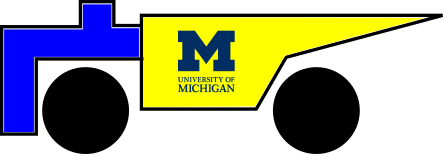
\includegraphics{Logo}

\noindent Tonka

\noindent Rishabh Shah

\noindent October 2, 2017

\noindent Bike Model: 1185}

\section*{Transmission}
\begin{table}[H]
	\centering
	\begin{tabular}{|r|c|c|c|}
		\hline
		\textbf{Gear} & \textbf{Diameter (inch)} & \textbf{Number of teeth} & \textbf{Circular Pitch}\\
		\hline
		One & 5 & 28 & 0.5610 \\
		\hline
		Two & 7 & 38 & 0.5787 \\
		\hline
		Three & 9 & 48 & 0.5890 \\
		\hline
	\end{tabular}
	\caption{Front gear assembly specifications}
\end{table}
\begin{table}[H]
	\centering
	\begin{tabular}{|r|c|c|c|}
		\hline
		\textbf{Gear} & \textbf{Diameter (inch)} & \textbf{Number of teeth} & \textbf{Circular Pitch} \\
		\hline
		One & 4 & 28 & 0.4488 \\
		\hline
		Two & \(3\frac{1}{2}\) & 24 & 0.4581 \\
		\hline
		Three & \(3\frac{1}{4}\) & 21 & 0.4862 \\
		\hline
		Four & 3 & 18 & 0.5236 \\
		\hline
		Five & \(2\frac{3}{4}\) & 16 & 0.5400 \\
		\hline
		Six & \(2\frac{1}{4}\) & 14 & 0.5049 \\
		\hline
	\end{tabular}
	\caption{Rear gear assembly specifications}
\end{table}
\begin{table}[H]
	\centering
	\begin{tabular}{|r|c|c|c|}
		\hline
		\textbf{Gear} & \textbf{Diameter (inch)} & \textbf{Number of teeth} & \textbf{Circular Pitch} \\
		\hline
		Upper & \(1\frac{3}{4}\) & 11 & 0.4998 \\
		\hline
		Lower & \(1\frac{3}{4}\) & 11 & 0.4988 \\
		\hline
	\end{tabular}
	\caption{Derailleur gear assembly specifications}
\end{table}
\begin{table}[H]
	\centering
	\begin{tabular}{|r|r|l|}
		\hline
		\textbf{Front gear} & \textbf{Rear gear} & \textbf{Gear Ratio} \\
		\hline
		One & One & 1.0000:1 \\
		One & Two & 1.1667:1 \\
		One & Three & 1.3333:1 \\
		One & Four & 1.5556:1 \\
		One & Five & 1.7500:1 \\
		One & Six & 2.0000:1 \\
		\hline
		Two & One & 1.3571:1 \\
		Two & Two & 1.5833:1 \\
		Two & Three & 1.8095:1 \\
		Two & Four & 2.1111:1 \\
		Two & Five & 2.3750:1 \\
		Two & Six & 2.7143:1 \\
		\hline
		Three & One & 1.7143:1 \\
		Three & Two & 2.0000:1 \\
		Three & Three & 2.2857:1 \\
		Three & Four & 2.6667:1 \\
		Three & Five & 3.0000:1 \\
		Three & Six & 3.4286:1 \\
		\hline
	\end{tabular}
	\caption{All possible gear ratios}
\end{table}

\section*{Linkages}
\begin{table}[H]
	\centering
	\begin{tabular}{|r|l|}
		\hline
		\textbf{Link or Joint} & \textbf{Length (inch)} \\
		\hline
		Front brake handle (long side) & \(3\frac{1}{4}\) \\
		\hline
		Front brake handle (short side) & 2 \\
		\hline
		Rear brake handle (long side) & \(3\frac{1}{4}\) \\
		\hline
		Rear brake handle (short side) & 2 \\
		\hline
		Front brake caliper & \(4{1}{2}\) \\
		\hline
		Front brake joint to pad & \(1\frac{1}{2}\) \\
		\hline
		Rear brake caliper & \(4{1}{2}\) \\
		\hline
		Rear brake joint to pad & \(1\frac{1}{2}\) \\
		\hline
	\end{tabular}
	\caption{Brake linkage specifications}
\end{table}

\section*{Bearings}
\begin{table}[H]
	\centering
	\begin{tabular}{|l|l|p{3.5in}|}
		\hline
		\textbf{Location} & \textbf{Type} & \textbf{Function} \\
		\hline
		Front axle & Radial ball bearing & Allow the front axle to turn freely and move the wheel \\
		\hline
		Rear axle & Radial ball bearing & Allow the rear axle to turn freely and move the wheel \\
		\hline
		Brake handle & Radial ball bearing & Allow the brake handle to be pulled smoothly during braking \\
		\hline
		Brake calipers & Radial ball bearing & Allow the brake caliper to turn freely when braking \\
		\hline
		Front sprocket & Radial ball bearing & Allow the front sprocket to turn freely while pedaling \\
		\hline
		Rear sprocket & Radial ball bearing & Allow the rear gear assembly to turn freely while pedaling \\
		\hline
		Derailleur tensioner & Radial ball bearing & Allow the derailleur to move freely when tensioning the chain \\
		\hline
		Derailleur gear change & Thrust ball bearing & Allow the derailleur to be at an angle from its mounting point so gears can be changed \\
		\hline
		Derailleur sprocket & Radial ball bearing & Allow the sprockets to turn freely while pedaling \\
		\hline
		Handlebars & Radial ball bearing & Allow the fork tube to turn freely while steering \\
		\hline
		Fork tube & Radial ball bearing & Allow the fork (attached to fork tube) to turn freely while steering \\
		\hline
	\end{tabular}
	\caption{Location, type, and functions of all bearings}
\end{table}

\end{document}